\section{The model}\label{sec:model}

\subsection{The car}
The car is described by its front overhang $d_f$, wheelbase $d_w$, rear overhang $d_b$, width $w$ (all positive) and maximal steering angle $\theta\in(0,\pi/2)$.
We write
\[
  R=\frac{d_w}{\tan\theta},\qquad b=d_w+d_f,\qquad \ell=b+d_b,\qquad \Rpm=R\pm\frac w2,
\]
\[
  \rho=\sqrt{b^2+\Rp^2},\qquad r=\sqrt{d_b^2+\Rp^2}.
\]
Here $b$ is the distance from the rear axle to the front bumper.
Throughout we assume
\begin{equation}\label{eq:standing}
  R>\tfrac w2,\qquad\text{i.e. } \Rm>0,
\end{equation}
which holds for every real car (typically $R\approx 2w$).

A \emph{configuration} is $q=(P,\psi)\in\R^2\times\R$, where $P=(P_x,P_y)$ is the midpoint of the rear axle and $\psi$ the heading.
We use the unit vectors
\[
  \e(\psi)=(\cos\psi,\sin\psi),\qquad \n(\psi)=(-\sin\psi,\cos\psi),
\]
which point forward and to the left.
In body coordinates the car occupies $\fp_0=[-d_b,b]\times[-\tfrac w2,\tfrac w2]$.
Its \emph{footprint} in configuration $q$ is
\[
  \fp(q)=\{P+u\,\e(\psi)+v\,\n(\psi):\ (u,v)\in\fp_0\}.
\]
We name the corners by the side of the car that faces the curb when the car is parked with heading $\psi\approx0$ (the right-hand side):
\[
  \cRC=P-d_b\e-\tfrac w2\n,\quad \cFC=P+b\e-\tfrac w2\n,\quad \cFL=P+b\e+\tfrac w2\n,\quad \cRL=P-d_b\e+\tfrac w2\n .
\]
Thus $\cRC$ is the rear corner on the curb side, $\cFL$ the front corner on the lane side, and so on.
When $\psi\in[0,\pi/2]$ the lowest point of the footprint is $\cRC$, the highest is $\cFL$, the leftmost is $\cRL$ and the rightmost is $\cFC$.
When $\psi\in[-\pi/2,0]$ these roles pass to $\cFC$, $\cRL$, $\cRC$ and $\cFL$ respectively.

\subsection{Kinematics and manoeuvres}
In the kinematic bicycle model the rear-axle midpoint moves tangentially to the car axis, and the heading turns at rate $\kappa$ per unit length of path, with $\kappa=\tan\omega/d_w$ for the steering angle $\omega\in[-\theta,\theta]$.
Hence $|\kappa|\le1/R$.
Speed plays no role, so we parametrise by arc length.

\begin{definition}[manoeuvre]\label{def:manoeuvre}
A \emph{manoeuvre} of direction $d\in\{+1,-1\}$ and length $S\ge0$ is a map $q=(P,\psi):[0,S]\to\R^2\times\R$ such that $\psi$ is Lipschitz with constant $1/R$ and
\[
  P(s)=P(0)+d\int_0^s\e(\psi(\sigma))\dd\sigma\qquad(0\le s\le S).
\]
Equivalently, $P$ is Lipschitz with $P'=d\,\e(\psi)$, and $|\psi'|\le1/R$ almost everywhere.
Forward motion is $d=+1$ and reverse motion is $d=-1$.
\end{definition}

The heading derivative is $\psi'=d\kappa$, so a measurable steering function corresponds exactly to a Lipschitz heading.
Full left lock means $\kappa=1/R$, i.e.\ $\psi'=d/R$; full right lock means $\psi'=-d/R$.
A \emph{motion with $n$ manoeuvres} is a concatenation of manoeuvres $q_1,\dots,q_n$ with $q_i(S_i)=q_{i+1}(0)$.
Two consecutive manoeuvres of the same direction can be merged, so the directions may be assumed to alternate, and zero-length manoeuvres are allowed.

\subsection{The slot}
Fix the margin $m\in(0,w)$ and put $H=m+w$.
For a slot length $L>0$, the curb, the parked car behind and the parked car in front are the open sets
\[
  \mathcal C=\{y<0\},\qquad \Or=(-\infty,0)\times(m,H),\qquad \Of=(L,\infty)\times(m,H).
\]
The \emph{free region} is $\Free=\R^2\setminus(\mathcal C\cup\Or\cup\Of)$.
We call the strip $\{m<y<H\}$ the \emph{band}.
The lane $\{y\ge H\}$ is unobstructed, and so is the gap $\{0\le y\le m\}$ between the parked cars and the curb.
The outer corners of the parked cars are
\[
  \Qr=(0,H),\qquad \Qf=(L,H),
\]
and their curb-side corners are $(0,m)$ and $(L,m)$.

\begin{definition}\label{def:fit}
A configuration $q$ is
\begin{itemize}[nosep]
\item \emph{free} if $\fp(q)\subset\Free$;
\item \emph{parked} (or \emph{fitting}) if it is free and $\fp(q)\subset\{y\le H\}$;
\item a \emph{lane configuration} if $\fp(q)\subset\{y\ge H\}$ and $\psi\in\pi\mathbb Z$.
\end{itemize}
A \emph{parking motion} (for the slot length $L$) is a motion that starts at a lane configuration, ends at a parked configuration, and passes only through free configurations.
Finally,
\[
  \Lmin(n)=\inf\{L>0:\ \text{a parking motion with at most $n$ manoeuvres exists}\}.
\]
\end{definition}

The parked cars are modelled as half-infinite strips, since only their ends adjacent to the slot can be touched.
The obstacles are open and the footprint is closed, so touching is allowed.
The ``fitting'' condition is the one requested in the problem: the point of the car closest to the open side of the road is no farther out than the sides of the cars in front and behind.
In the main application $m=w/10$.

\begin{figure}[ht]
\centering
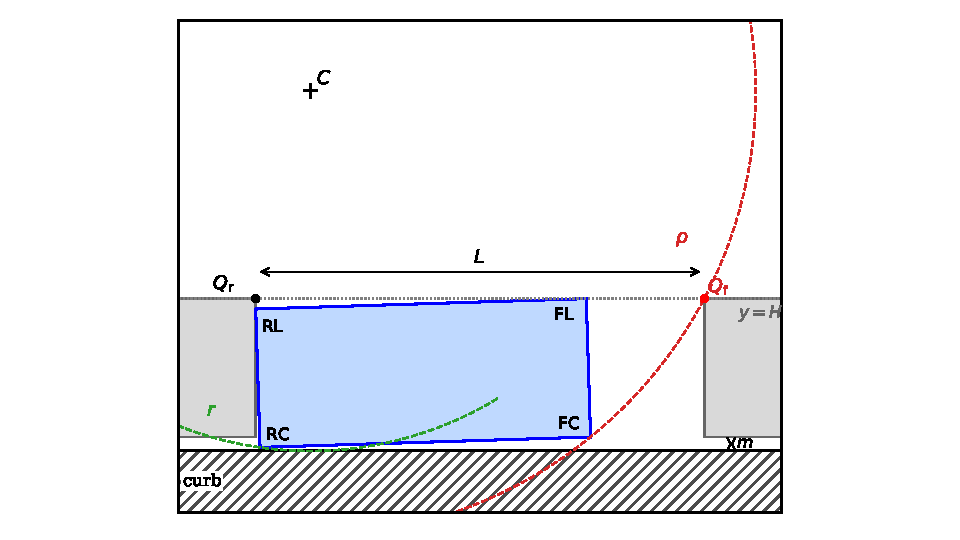
\includegraphics[width=0.85\textwidth]{figures/fig_geometry.pdf}
\caption{The slot (typical car, $L=\Lambda_1$).
The parked cars (grey) occupy $m\le y\le H$; the curb is hatched.
Our car is shown in the optimal one-manoeuvre position $q_d$ of \cref{thm:one}.
Under full left lock it rotates about $C$: the front curb-side corner $\cFC$ moves on the circle of radius $\rho$ through $\Qf$ (red), and the rear curb-side corner $\cRC$ on the circle of radius $r$ tangent to the curb (green).}
\label{fig:geometry}
\end{figure}

\subsection{Elementary properties}

\begin{lemma}[time reversal]\label{lem:reversal}
If $q$ is a manoeuvre of direction $d$ and length $S$, then $\tilde q(s)=q(S-s)$ is a manoeuvre of direction $-d$.
Consequently, a parking motion with $n$ manoeuvres exists if and only if an \emph{exit motion} with $n$ manoeuvres exists, i.e.\ a free motion from a parked configuration to a lane configuration.
\end{lemma}
\begin{proof}
$\tilde\psi(s)=\psi(S-s)$ is $1/R$-Lipschitz, and
\[
  \tilde P(s)=P(S)-d\int_{S-s}^{S}\e(\psi)=\tilde P(0)+(-d)\int_0^s\e(\tilde\psi(\sigma))\dd\sigma.
\]
Reversing the order of the manoeuvres of a parking motion gives an exit motion and conversely.
\end{proof}

From now on we mostly work with exits, which are easier to visualise: the car drives \emph{out} of the slot.

\begin{lemma}[monotonicity]\label{lem:monoL}
If $L\le L'$ then $\Free\subset\mathcal F_{L'}$; hence free, parked and lane configurations for $L$ are also free, parked and lane configurations for $L'$.
The set of slot lengths admitting a parking motion with at most $n$ manoeuvres is therefore an up-set.
Moreover $\Lmin(n+1)\le\Lmin(n)$.
\end{lemma}
\begin{proof}
Only $\Of$ depends on $L$, and it shrinks as $L$ grows.
A motion with at most $n$ manoeuvres also has at most $n+1$.
\end{proof}

\begin{lemma}[mirror symmetry]\label{lem:mirror}
The map $\mu_L(x,y,\psi)=(L-x,\,y,\,\pi-\psi)$ satisfies $\fp(\mu_L q)=\sigma(\fp(q))$ for the reflection $\sigma(x,y)=(L-x,y)$.
It maps manoeuvres to manoeuvres of the same direction and preserves the classes of free, parked and lane configurations.
\end{lemma}
\begin{proof}
The linear part of $\sigma$ sends $\e(\psi)$ to $\e(\pi-\psi)$ and $\n(\psi)$ to $-\n(\pi-\psi)$.
Since $\fp_0$ is symmetric under $v\mapsto -v$, $\sigma(\fp(P,\psi))=\fp(\sigma P,\pi-\psi)$.
Also $(\sigma P)'=d\,\e(\pi-\psi)$, so $\mu_L$ maps manoeuvres to manoeuvres of the same direction.
Finally $\sigma$ preserves $\mathcal C$ and the lane, and swaps $\Or$ and $\Of$.
\end{proof}

\begin{lemma}[parked cars are nearly level]\label{lem:fit}
Assume $H<\ell$ and let $\psi_{\rm fit}\in(0,\arctan(\ell/w))$ be the root of $\ell\sin\psi+w\cos\psi=H$.
If $q$ is parked, then $\psi$ lies within $\psi_{\rm fit}$ of a multiple of $\pi$.
\end{lemma}
\begin{proof}
The vertical extent of the footprint is $\ell|\sin\psi|+w|\cos\psi|$, and it must be at most $H$.
On $[0,\pi/2]$ the function $f(\psi)=\ell\sin\psi+w\cos\psi$ increases from $w<H$ to $\sqrt{\ell^2+w^2}$ and then decreases to $\ell>H$.
Hence $\{f\le H\}\cap[0,\pi/2]=[0,\psi_{\rm fit}]$, and the other quadrants follow by symmetry.
\end{proof}

Shifting the heading by a multiple of $2\pi$ changes nothing, and \cref{lem:mirror} maps headings near odd multiples of $\pi$ to headings near even ones.
We may and do therefore assume that the parked configuration at which an exit starts has $|\psi|\le\psi_{\rm fit}$.

\subsection{A soft curb}\label{sec:model-soft}
Ordinary curbs are lower than the bumpers and sills of a car.
The bodywork may then overhang the curb, and only the tyres have to stay on the road.
We call this the \emph{soft-curb model}, and the model above the \emph{rigid-curb model}.
In plan view each tyre is a rectangle aligned with the car, and in body coordinates the four tyres occupy
\[
  \W_0=\big([-\lambda,\lambda]\cup[d_w-\lambda,d_w+\lambda]\big)\times\big([-T_o,-T_o+t_w]\cup[T_o-t_w,T_o]\big).
\]
Here $\lambda$ is half the length of a tyre, $t_w$ its width and $T_o$ the distance of the outer sidewalls from the axis of the car.
We assume $\W_0\subset\fp_0$, i.e.\ $\lambda\le\min(d_b,d_f)$ and $T_o\le w/2$, and write $\delta_s=w/2-T_o\ge0$ for the inset of the outer sidewalls.

In the soft-curb model a configuration $q$ is \emph{free} if $\fp(q)\cap(\Or\cup\Of)=\emptyset$ and $\W(q)\cap\mathcal C=\emptyset$, where $\W(q)$ is the image of $\W_0$ under the rigid motion that maps $\fp_0$ to $\fp(q)$.
Parked and lane configurations, parking motions and the minimal length $\Lmins(n)$ are defined as in \cref{def:fit}, with this notion of freeness.
A parked car may therefore overhang the curb, but it must still lie in $\{y\le H\}$.
Since $\W_0\subset\fp_0$, every configuration that is free in the rigid-curb model is free in the soft-curb model, and hence
\begin{equation}\label{eq:soft-le}
  \Lmins(n)\le\Lmin(n)\qquad\text{for every }n.
\end{equation}
\Cref{lem:reversal,lem:monoL} hold verbatim, and so does \cref{lem:mirror}, because $\W_0$ is symmetric under $v\mapsto-v$.

For numerical values we use the same tyres for every car: $\delta_s=0.0275$ m, $t_w=0.205$ m and $\lambda=0.25$ m.
This is a $205$ mm tyre whose outer sidewall is $2.75$ cm inside the body side, and $2\lambda$ is the chord of a tyre of diameter $0.63$ m at a curb height of $0.12$ m.
We do not turn the front tyres with the steering.
All motions behind our numerical values remain free when the front tyres are turned to the Ackermann angles of full lock (\cref{app:numerics}), so the upper bounds hold in that model too.
The soft-curb model is analysed in \cref{sec:soft}, and the two models are compared in \cref{sec:compare}.
